\documentclass[10pt,fleqn]{article} % Default font size and left-justified equations
\usepackage[%
    pdftitle={CIN : Vérification des performances cinématiques des systèmes},
    pdfauthor={Xavier Pessoles}]{hyperref}
    
\input{style/new_style}
\input{style/macros_SII}

\usepackage{multicol}
\fichetrue
%\fichefalse

\proftrue
%\proffalse

\tdtrue
%\tdfalse

\courstrue
\coursfalse

\def\discipline{Sciences \\Industrielles de \\ l'Ingénieur}
\def\xxtete{Sciences Industrielles de l'Ingénieur}

\def\classe{PTSI}
\def\xxnumpartie{Cycle 8}
\def\xxpartie{Vérification des performances cinématiques des systèmes\\
Analyser, Modéliser, Résoudre}

\def\xxnumchapitre{Chapitre 5}
\def\xxchapitre{Étude des trains épicycloïdaux}

\def\xxtitreexo{Centrifugeuse des boues d'une station d'épuration.}
\def\xxsourceexo{\hspace{.2cm} D'après concours CCP -- MP 2012.}


\def\xxposongletx{2}
\def\xxposonglettext{1.45}
\def\xxposonglety{20}
\def\xxonglet{Cycle 6 -- Ch. 5}

\def\xxactivite{Colle 4}
\def\xxauteur{\textsl{Xavier Pessoles}}

\def\xxcompetences{%
\textsl{%
\textbf{Savoirs et compétences :}\\
\noindent \textbf{Analyser :} 
\begin{itemize}[label=\ding{112},font=\color{ocre}] 
\item \textit{A3 -- C6 :} transmetteurs de puissance.
\end{itemize}
\noindent \textbf{Modéliser :} \textit{proposer un modèle de connaissance du système.}
}}

\def\xxfigures{
\includegraphics[width=.7\textwidth]{images/centrifugeuse_01}
}%figues de la page de garde

\def\xxpied{%
Cycle 6 -- Vérification des performances cinématiques \\
Ch. 5 : Étude des trains épicycloïdaux -- \xxactivite%
}


\setcounter{secnumdepth}{5}
%---------------------------------------------------------------------------


\begin{document}
%\chapterimage{png/Fond_Cin}
\input{style/new_pagegarde}
\vspace{7cm}
\pagestyle{fancy}
\thispagestyle{plain}


\def\columnseprulecolor{\color{ocre}}
\setlength{\columnseprule}{0.4pt} 

\begin{multicols}{2}

\begin{obj} Déterminer la vitesse d'un moteur pour répondre au cahier des charges. 
\end{obj}

\footnotesize{
\textit{Les boues sont constituées d’eau et de matière sèche. La siccité est le pourcentage massique de matière
sèche. Ainsi, une boue avec une siccité de 10\% présente une humidité de 90\%. Afin
d’incinérer les boues, il faut les déshydrater pour atteindre une siccité de 20\%. La déshydratation
mécanique par centrifugation permet de séparer l’eau des matières sèches dans les boues.
La centrifugation se base sur la différence de densité entre les matières sèches et l’eau présente dans
cette boue. La boue arrive avec une certaine vitesse horizontale par un coté de la centrifugeuse. L’eau 
traverse alors toute la centrifugeuse dans sa
zone centrale tandis que les matières en suspension sont plaquées contre le tambour extérieur du fait
de sa vitesse de rotation. Une vis intérieure, tournant dans le même sens que le tambour mais à une
vitesse plus importante, vient alors récupérer les boues et les évacuer en sens inverse de l’eau jusqu’à
la sortie latérale.}}

\begin{center}
\includegraphics[width=\linewidth]{images/centrifugeuse_02}
\end{center}

La boue visqueuse est cisaillée par la différence de vitesse entre la vis et le tambour (bol extérieur).
La siccité de la boue est directement liée à cette différence de vitesse. On donne le diagramme des exigences partiel :

\begin{center}
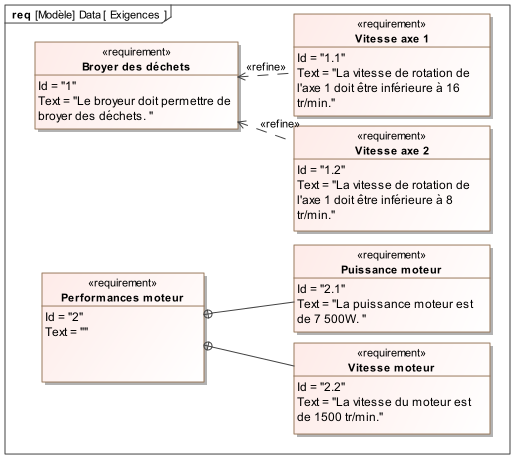
\includegraphics[width=.8\linewidth]{images/Exigences}
\end{center}


La chaîne cinématique est représentée sur la figure
suivante.

\begin{center}
\includegraphics[width=\linewidth]{images/centrifugeuse_03}
\end{center}






La séquence de lancement de la centrifugeuse se déroule en trois phases :
\begin{itemize}
\item mise en marche du premier moteur $M_{\text{tambour}}$ jusqu’à ce que le tambour 1 atteigne sa vitesse
de consigne de 2 000 tours/min. Le moteur $M_{\text{rel}}$ est à l’arrêt;
\item mise en marche du deuxième moteur $M_{\text{rel}}$ jusqu’à ce que la vitesse différentielle de
2 tours/min soit atteinte entre le tambour 1 et la vis 3. La vis 3 tourne ainsi plus vite que le
tambour 1;
\item la boue liquide est ensuite introduite.
\end{itemize}

\subparagraph{}
\textit{Déterminer la fréquence de rotation de la vis (par rapport au bâti) lors de la phase de lancement.}

\subparagraph{}
\textit{Déterminer alors la fréquence de rotation que doit avoir le moteur <<rel>> pour respecter l'exigence 1.1.}
\end{multicols}

\end{document}


